\documentclass{beamer}


\usetheme{Madrid}
\usecolortheme{default}


% --- PREAMBLE: PACKAGES AND DOCUMENT INFO ---
\usepackage[utf8]{inputenc}
\usepackage[T1]{fontenc}
\usepackage{amsmath}
\usepackage{amsfonts}
\usepackage{amssymb}
\usepackage{hyperref}
\usepackage{tikz}
\usepackage{subcaption}

\usetikzlibrary{arrows.meta}
\tikzset{
    dot/.style={circle, fill, inner sep=1.5pt}, % 定义格点的样式
    main plot/.style={scale=0.7, font=\small} % 定义每个子图的通用样式
}

\usefonttheme{professionalfonts} % 允许更自由的字体尺寸设置
\AtBeginDocument{\small} % 在文档开始时全局应用 small 字体

% --- 全局行间距设置 ---
\usepackage{setspace}
\setstretch{1.2} % 全局设置行间距为1.2倍

\newcommand{\ket}[1]{\left| #1 \right\rangle}
\newcommand{\vev}[1]{\left\langle #1 \right\rangle}


% --- Fill in your information here ---
\title[The \texorpdfstring{$\widetilde{SL}_{2}(\mathbb{R})$}{Lg} WZW Model]{Degenerate Representations and Fusion Rules in the $\widetilde{SL}_{2}(\mathbb{R})$ WZW Model}

% The \author command can hold your name.
% The optional [short name] is for the footer if your name is long.
\author[Hexuan Li]{Hexuan Li}

% The \institute command can hold your university and advisor information.
\institute[École Polytechnique]
{
  
  Advisor: Prof. Sylvain Ribault
}

% The \date command sets the date on the title page. \today is automatic.
\date{\today}


% --- BEGIN DOCUMENT ---
\begin{document}

% --- TITLE PAGE FRAME ---
% The [plain] option removes the header and footer for a clean title page.
\begin{frame}[plain]
  \titlepage
\end{frame}

\begin{frame}{Contents}
  \tableofcontents
\end{frame}

\section{Introduction}

\begin{frame}{String theory on AdS\texorpdfstring{${}_{3}$}{Lg}}
  \begin{itemize}
    \item The AdS/CFT correspondence is a powerful tool, which relats gravity in an Anti-de Sitter (AdS) spacetime with a conformal field 
    theory (CFT) that lives on its boundary.
    \vspace{0.5cm}
    \item We are interested in string theory on AdS${}_{3}$, since: 
      \begin{itemize}
        \item Understanding string theory in AdS${}_{3}$ enables us to study the AdS/CFT correspondence beyond gravity approximation. 
        \item It describes string theory on a curved spacetime, where the $g_{00}$ component of metric is non-trivial.
      \end{itemize}
    \vspace{0.5cm}
    
    \item String theory on AdS${}_{3}$ is described by the $\widetilde{SL}_{2}(\mathbb{R})$ Wess-Zumino-Witten (WZW) 
    model. 

  \end{itemize}
\end{frame}

\begin{frame}{\texorpdfstring{$\widetilde{SL}_{2}(\mathbb{R})$}{Lg} WZW model}
  \begin{itemize}
    \item The $\widetilde{SL}_{2}(\mathbb{R})$ is a conformal field theory(CFT) with an $\widehat{\mathfrak{sl}}_{2}$ symmetry. 
    \item The model has not been completely solved. The three-point functions are not fully known, and crossing symmetry has not been 
    proved yet.
    \item In order to use conformal bootstrap to solve this model, we need the fusion rules for the representations of 
    $\widehat{\mathfrak{sl}}_{2}$.
    \vspace{1cm}
    \begin{block}{}
      In this presentation, we are going to give some of the fusion rules 
      between degenerate representations and affine highest representations.
    \end{block}
  \end{itemize}
\end{frame}

\section{\texorpdfstring{$\widetilde{SL}_{2}(\mathbb{R})$}{Lg} WZW model}

\begin{frame}{Symmetry algebra}
  \begin{itemize}
    \item The $\widehat{\mathfrak{sl}}_{2}$ algebra is generated by 3 holomorphic currents $J^{a}(z)$ through their operator product expansions (OPE), 
      \begin{equation}
        J^{a}(z)J^{b}(w) = \frac{kK^{ab}}{(z-w)^{2}} + \frac{f^{ab}_{c} J^{c}(w)}{z-w} + \mathcal{O}(1), \label{OPEJJ}
      \end{equation}
    where the constant $k$ is the level, $K^{ab}$ is the Killing tensor $K^{ab} = \frac{1}{2g} f^{ac}_{d}f^{bd}_{c}$.
    \item The generators of $\widehat{\mathfrak{sl}}_{2}$ algebra are defined as 
    $J^{a}_{n} = \oint \mathrm{d}z \, z^{n} J^{a}(z)$.
    We deduce the following commutation relations from the OPE
      \begin{equation}
          \left[ J^{a}_{m}, J^{b}_{n} \right] = f^{ab}_{c} J^{c}_{m+n} + m k K^{ab} \delta_{m+n,0}. 
      \end{equation}
    \item We introduce the Sugawara construction of the Virasoro generators:
      \begin{equation}
        L_{n} = \frac{K_{ab}}{2(k-2)} : \sum_{m \in \mathbb{Z} } J^{a}_{n-m} J^{b}_{m} :.
      \end{equation}
  \end{itemize}
\end{frame}

\begin{frame}{Spectral flow}
  \begin{itemize}
    \item The spectral flow is a family $(\rho_{\omega})_{\omega \in \mathbb{Z}}$ of automorphisms of $\widehat{\mathfrak{sl}}_{2}$
      satisfying $\rho_{\omega_{1}} \circ \rho_{\omega_{2}}  = \rho_{\omega_{1} + \omega_{2}}$, which are defined by 
      \begin{equation}
          \begin{aligned}
              \rho_{\omega}(J^{\pm}_{m}) & = J^{\pm}_{m \pm \omega},\\
              \rho_{\omega}(J^{0}_{m}) & = J^{0}_{m} + \frac{1}{2} k \omega \delta_{m,0}.
          \end{aligned}
      \end{equation}
    \item The spectral flow of Virasoro generators is 
      \begin{equation}
          \rho_{\omega}(L_{m}) = L_{m} + \omega J^{0}_{m} + \frac{1}{4} k n^{2} \delta_{m,0}.
      \end{equation}
  \end{itemize}
\end{frame}

\begin{frame}{Affine primary fields}
  \begin{itemize}
    \item An affine primary field $\phi^{j}(z)$ associated with representation $\mathcal{R}^{j}$ is defined by its OPE with current field 
      $J^{a}(y)$:
      \begin{equation}
        J^{a}(y) \phi^{j}(z) \sim \frac{-(t^{a})^{T} \phi^{j}(z)}{y-z} + \mathcal{O}(1), \label{OPEJPhi}
      \end{equation}
      where $t^{a}$ is the generator of Lie algebra $\mathfrak{sl}_{2}$.
    \item The conformal dimension of $\phi^{j}(z)$ is propotional to the Casimir operator $C = K_{ab} t^{a} t^{b} = 2j(j+1)$ :
      \begin{equation}
        \Delta_{j} = \frac{C(j)}{2(k-2)} = \frac{j(j+1)}{k-2}.
      \end{equation}
  \end{itemize}
\end{frame}

\begin{frame}{Isospin variables}
    
  \begin{itemize}
    \item We introduce the isospin variables and represent the fields as functions of the isospin variables, 
          where $t^{a}$ acts on primary fields as differential operators $D^{j}(t^{a})$. 
    \item A field is represented as a function $\phi^{j}_{x}$ of $x$, and $t^{a}$ acts as 
      \begin{equation}
          \left\{
              \begin{aligned}
                  D^{j}_{x}(t^{+}) &= x^{2} \partial_{x} - 2 j x, \\
                  D^{j}_{x}(t^{0}) &= x \partial_{x} - j, \\
                  D^{j}_{x}(t^{-}) &= - \partial_{x}.
              \end{aligned}
          \right. \label{Diffx}
      \end{equation}
  \end{itemize}
\end{frame}

\begin{frame}{\texorpdfstring{$m$}{Lg}-basis}
  \begin{itemize}
    \item Another important basis is the $m$-basis, where $J^{0}_{0}$ is diagonalized. 
          $J^{a}_{0}$ act on the $m$-basis fields as 
      \begin{equation}
          \left\{
              \begin{aligned}
                  J^{+}_{0} \phi^{j}_{m} &= (j-m) \phi^{j}_{m+1}, \\
                  J^{0}_{0} \phi^{j}_{m} &= m \phi^{j}_{m},\\
                  J^{-}_{0} \phi^{j}_{m} &= (j+m) \phi^{j}_{m-1}.
              \end{aligned}
          \right. \label{Diffm}
      \end{equation}
    \item The fields in the $m$-bases and $x$-basis are related by
          \begin{equation}
              \phi^{j}_{m}(z) \sim \int \mathrm{d} x \, x^{j+m} \phi^{j}_{x}(z).
          \end{equation}
  \end{itemize}
\end{frame}

\begin{frame}{Irreducible representations of \texorpdfstring{$\mathfrak{sl}_{2}$}{Lg}}
  \begin{itemize}
    \item A representation $\mathcal{R}$ of $\mathfrak{sl}_{2}$ can be extended to an affine highest-weight representation 
      $\widehat{\mathcal{R}}$ by acting with creation operators $J^{a}_{n<0}$.
    \item We classify the irreducible representations of $\mathfrak{sl}_{2}$ into the following series:
      \begin{itemize}
        \item Principle continuous series $\mathcal{C}^{j}_{\alpha}, \ j \in -\frac{1}{2} + i \mathbb{R}_{+}$. 
        \item Discrete series $\mathcal{D}^{j,\pm}, \ j \in (- \infty, - \frac{1}{2})$. 
        \item Finite dimensional representations $\mathcal{E}^{j},\ j\in \mathbb{N}/2$.
      \end{itemize}
      The representations can be characterized by the eigenvalues $m$ of $J^{0}_{0}$.
  \end{itemize}
  \vspace{0.5cm}
  \begin{center}
    \begin{tabular}{|l|l|l|}
        \hline
        Representations&Parameter values&Eigenvalues of $J^{0}_{0}$\\
        \hline
        $\mathcal{C}^{j}_{\alpha}$ & $j \in -\frac{1}{2} + i \mathbb{R}_{+} $, $\alpha \in \mathbb{R}$ mod $\mathbb{Z}$& $\alpha + \mathbb{Z}$\\
        $\mathcal{D}^{j,+}$ & $j \in (-\infty,-\frac{1}{2}) $& $-j + \mathbb{N}$\\
        $\mathcal{D}^{j,-}$ & $j \in (-\infty,-\frac{1}{2}) $& $j - \mathbb{N}$\\
        $\mathcal{E}^{j}$ & $j \in \mathbb{N}/2 $ & $\left\{-j,-j+\frac{1}{2}, \cdots, j-\frac{1}{2},j \right\}$\\
        \hline
    \end{tabular}
\end{center}
\end{frame}

\begin{frame}{Irreducible representations of \texorpdfstring{$\mathfrak{sl}_{2}$}{Lg}}
  \begin{figure}[h]
    \centering 
        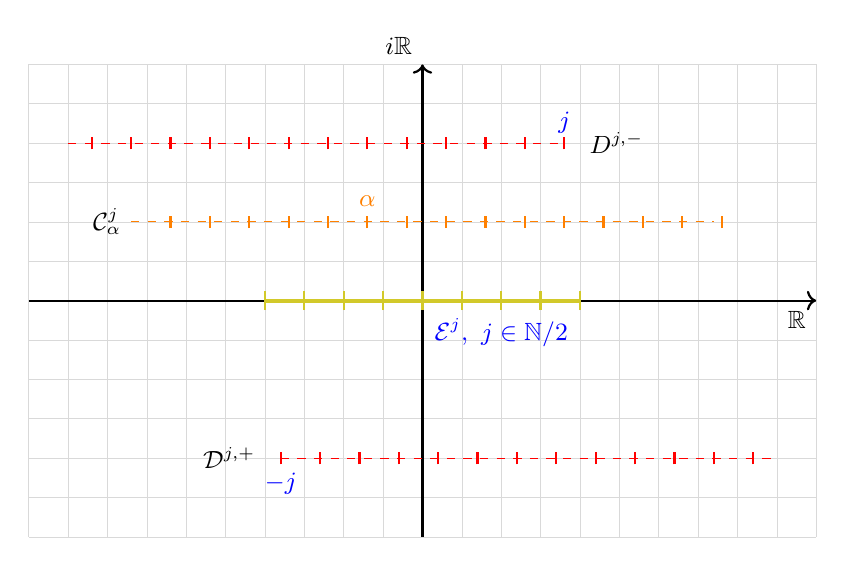
\begin{tikzpicture}[
    x=1cm, y=1cm, % 定义坐标单位长度
    font=\small
    ]
    % --- 定义绘图区域 ---
    \def\xmin{-5} \def\xmax{5}
    \def\ymin{-3} \def\ymax{3}
    \def\ticksize{0.08cm} % 定义刻度线的半长

    % 1. 绘制背景网格
    \draw[help lines, color=gray!30, step=0.5] (\xmin, \ymin) grid (\xmax, \ymax);

    % 2. 绘制坐标轴
    \draw[->, thick] (\xmin, 0) -- (\xmax, 0) node[below left] {$\mathbb{R}$};
    \draw[->, thick] (0, \ymin) -- (0, \ymax) node[above left] {$i\mathbb{R}$};
    
    % --- 绘制四条带刻度的线及其标签 ---
    
    % a) 顶部的红色线
    \begin{scope}[yshift=2cm]
        % 绘制虚线
        \draw[red, dashed] (-4.5, 0) -- (1.8, 0);
        % 绘制刻度
        \foreach \x in {-4, -3.5, ..., 2} {
            \draw[red, thick] (\x-0.2, -\ticksize) -- (\x-0.2, \ticksize);
        }
        % 添加标签
        \node[blue, above] at (1.8, 0) {$j$};
        \node[black, right] at (2.0, 0) {$D^{j,-}$};
    \end{scope}

    % b) 中间的橙色线
    \begin{scope}[yshift=1cm]
        \draw[orange, dashed] (-3.7, 0) -- (3.7, 0);
        \foreach \x in {-3.5, -3, ..., 3.5} {
            \draw[orange, thick] (\x+0.3, -\ticksize) -- (\x+0.3, \ticksize);
        }
        \node[black, left] at (-3.7, 0) {$\mathcal{C}^{j}_{\alpha}$};
        \node[orange, above=2pt] at (-0.7, 0) {$\alpha$};
    \end{scope}
    
    % c) 坐标轴上的黄色线
    \begin{scope}[yshift=0cm]
        % 这条线看起来更实一些
        \draw[yellow!80!black, line width=1.5pt] (-2, 0) -- (2, 0);
        \foreach \x in {-2, -1.5, ..., 2} {
            \draw[yellow!80!black, thick] (\x, -\ticksize*1.5) -- (\x, \ticksize*1.5);
        }
        \node[blue, below=3pt] at (1, 0) {$\mathcal{E}^{j},\ j\in \mathbb{N}/2$};
    \end{scope}

    % d) 底部的红色线
    \begin{scope}[yshift=-2cm]
        \draw[red, dashed] (-1.8, 0) -- (4.5, 0);
        \foreach \x in {-2, -1.5, ..., 4} {
            \draw[red, thick] (\x+0.2, -\ticksize) -- (\x+0.2, \ticksize);
        }
        \node[black, left] at (-2.0, 0) {$\mathcal{D}^{j,+}$};
        \node[blue, below=2pt] at (-1.8, 0) {$-j$};
    \end{scope}

    \end{tikzpicture}
    \caption{The spectra of irreducible representations of $\mathfrak{sl}_{2}$}
    \label{fig:sl2}
  \end{figure}
\end{frame}


\begin{frame}[c]{Affine highest-weight representations of \texorpdfstring{$\widehat{\mathfrak{sl}}_{2}$}{Lg}}
\begin{figure}
    \centering
    \def\tikzscale{0.5} 

    \begin{subfigure}[b]{0.48\textwidth}
        \centering
        \begin{tikzpicture}[scale=\tikzscale, font=\small] % 使用定义的 scale
            \def\xmin{-4.5} \def\xmax{4.5} \def\ymin{-2.5} \def\ymax{4.5}
            \clip (\xmin-1, \ymin) rectangle (\xmax+1, \ymax+1);
            \fill[violet!20] (\xmin, 0) rectangle (\xmax, \ymax);
            \draw[-{Stealth[]}] (\xmin, 0) -- (\xmax, 0) node[anchor=north west, xshift=-15pt] {$J_0^0/m$};
            \draw[-{Stealth[]}] (0, \ymin) -- (0, \ymax) node[anchor=south east] {$L_0/\Delta$};
            \foreach \x in {-4,...,4} {\foreach \y in {-2,...,4} {\node[dot] at (\x+0.2,\y) {};}}
            \node[draw, fill=white, rounded corners=2pt, align=left, anchor=north east, font=\tiny] at (\xmax-0.2, \ymax-0.2) {
                \begin{tabular}{rl}\tikz\fill[violet!20](0,0)rectangle(0.2,0.2);&Allowed states\end{tabular}};
        \end{tikzpicture}
        \caption{$\widehat{\mathcal{C}}^{j}_{\alpha}$}
        \label{fig:C}
    \end{subfigure}
    \hfill
    \begin{subfigure}[b]{0.48\textwidth}
        \centering
        \begin{tikzpicture}[scale=\tikzscale, font=\small] 
            \def\xmin{-4.5} \def\xmax{4.5} \def\ymin{-2.5} \def\ymax{4.5}
            \clip (\xmin-1, \ymin) rectangle (\xmax+1, \ymax+1);
            \fill[violet!20] (\xmin, -\xmin-1) -- (-1, 0) -- (1, 0) -- (\xmax, \xmax-1) -- (\xmax, \ymax) -- (\xmin, \ymax) -- cycle;
            \draw[-{Stealth[]}] (\xmin, 0) -- (\xmax, 0) node[anchor=north west, xshift=-15pt] {$J_0^0/m$};
            \draw[-{Stealth[]}] (0, \ymin) -- (0, \ymax) node[anchor=south east] {$L_0/\Delta$};
            \foreach \x in {-4,...,4} {\foreach \y in {-2,...,4} {\node[dot] at (\x,\y) {};}}
            \node[draw, fill=white, rounded corners=2pt, align=left, anchor=north east, font=\tiny] at (\xmax-0.2, \ymax-0.2) {
                \begin{tabular}{rl}\tikz\fill[violet!20](0,0)rectangle(0.2,0.2);&Allowed states\end{tabular}};
        \end{tikzpicture}
        \caption{$\widehat{\mathcal{E}}^{j}$}
        \label{fig:E}
    \end{subfigure}
    

    \caption{The spectra of irreducible representations of $\widehat{\mathfrak{sl}_{2}} (1)$}
    \label{fig:irrep1}
\end{figure}
\end{frame}

\begin{frame}[c]{Affine highest-weight representations of \texorpdfstring{$\widehat{\mathfrak{sl}}_{2}$}{Lg}}
\begin{figure}
    \centering
    \def\tikzscale{0.5} 
    \begin{subfigure}[b]{0.48\textwidth}
        \centering
        \begin{tikzpicture}[scale=\tikzscale, font=\small] 
            \def\xmin{-4.5} \def\xmax{4.5} \def\ymin{-2.5} \def\ymax{4.5}
            \clip (\xmin-1, \ymin) rectangle (\xmax+1, \ymax+1);
            \fill[violet!20] (\xmin, -\xmin-1.2) -- (-1.2, 0) -- (\xmax, 0) -- (\xmax, \ymax) -- (\xmin, \ymax) -- cycle;
            \draw[-{Stealth[]}] (\xmin, 0) -- (\xmax, 0) node[anchor=north west, xshift=-15pt] {$J_0^0/m$};
            \draw[-{Stealth[]}] (0, \ymin) -- (0, \ymax) node[anchor=south east] {$L_0/\Delta$};
            \foreach \x in {-4,...,4} {\foreach \y in {-2,...,4} {\node[dot] at (\x-0.2,\y) {};}}
            \node[draw, fill=white, rounded corners=2pt, align=left, anchor=north east, font=\tiny] at (\xmax-0.2, \ymax-0.2) {
                \begin{tabular}{rl}\tikz\fill[violet!20](0,0)rectangle(0.2,0.2);&Allowed states\end{tabular}};
        \end{tikzpicture}
        \caption{$\widehat{\mathcal{D}}^{j,+}$}
        \label{fig:D+}
    \end{subfigure}
    \hfill
    \begin{subfigure}[b]{0.48\textwidth}
        \centering
        \begin{tikzpicture}[scale=\tikzscale, font=\small] % 使用定义的 scale
            \def\xmin{-4.5} \def\xmax{4.5} \def\ymin{-2.5} \def\ymax{4.5}
            \clip (\xmin-1, \ymin) rectangle (\xmax+1, \ymax+1);
            \fill[violet!20] (\xmin, 0) -- (1.2, 0) -- (\xmax, \xmax-1.2) -- (\xmax, \ymax) -- (\xmin, \ymax) -- cycle;
            \draw[-{Stealth[]}] (\xmin, 0) -- (\xmax, 0) node[anchor=north west, xshift=-15pt] {$J_0^0/m$};
            \draw[-{Stealth[]}] (0, \ymin) -- (0, \ymax) node[anchor=south east] {$L_0/\Delta$};
            \foreach \x in {-4,...,4} {\foreach \y in {-2,...,4} {\node[dot] at (\x+0.2,\y) {};}}
            \node[draw, fill=white, rounded corners=2pt, align=left, anchor=north east, font=\tiny] at (\xmax-0.2, \ymax-0.2) {
                \begin{tabular}{rl}\tikz\fill[violet!20](0,0)rectangle(0.2,0.2);&Allowed states\end{tabular}};
        \end{tikzpicture}
        \caption{$\widehat{\mathcal{D}}^{j,-}$}
        \label{fig:D-}
    \end{subfigure}

    \caption{The spectra of irreducible representations of $\widehat{\mathfrak{sl}_{2}} (2)$}
    \label{fig:irrep2}
\end{figure}
\end{frame}

\begin{frame}{Spectral flowed representations}
  \begin{itemize}
    \item A representation $\widehat{\mathcal{R}} $ provides the action of generators $J^{a}_{n}$ on vector space $V$. 
    \item The spectral flowed representation $\rho_{\omega}\left(\hat{\mathcal{R}}\right)$ acts on the 
          vector space $V_{\omega} = \left\{ \left|v, \omega \right\rangle \Big| \left|v \right\rangle \in V \right\}$, 
          where the action of generators is defined to be 
          \begin{equation}
            J^{a}_{n} \left|v, \omega \right\rangle = \rho_{-\omega}\left(J^{a}_{n}\right) \left|v \right\rangle
          \end{equation}
    \item The conformal dimension of states in $\rho_{\omega} \left(\hat{\mathcal{C}}^{j}\right), \omega \neq 0$ are not bounded 
      from below. Hence it cannot be an affine highest-weight representation.
    \item On the other hand, we have 
      \begin{equation}
        \begin{aligned}
            \rho_{-1}\left( \widehat{\mathcal{D}}^{j,+} \right) &= \widehat{\mathcal{D}}^{\frac{k}{2}-j,-}\\
            \rho_{1}\left( \widehat{\mathcal{D}}^{j,-} \right) &= \widehat{\mathcal{D}}^{\frac{k}{2}-j,+}\\
        \end{aligned}
      \end{equation}
  \end{itemize}
\end{frame}

\section{Degenerate representations}

\begin{frame}{Degenerate representations}
  \begin{itemize}
    \item A descendant state $\ket{\chi} = \hat{N} \ket{j_{\hat{N}}} $ is called a null vector if it is annihilated by all 
    the positive modes:
      \begin{equation}
          J^{a}_{n>0} \ket{\chi} = 0, \label{nullvectoreq}
      \end{equation}
    \item The null vector and its descendants form a non-trivial submodule $\widehat{\mathcal{V}}'$ of the representation $\widehat{\mathcal{V}}^{j}$.
    A degenerate representation is obtained by taking the quotient of the Verma module by this submodule:
      \begin{equation}
          \widehat{\mathcal{R}}^{j} = \widehat{\mathcal{V}}^{j} / \widehat{\mathcal{V}}'
      \end{equation}
    \item The degenerate representations $\widehat{\mathcal{R}}^{\vev{r,s}}$ are labeled by two integer $r$ and $s$, whose null vector 
      lives at level $N = rs$. The corresponding spin $j_{r,s}$ is given by: 
      \begin{equation}
          j_{r,s} = \frac{s-1}{2} - \frac{k+2}{2} r \quad \mathrm{for} \quad s\geq 1, r \geq 0.
      \end{equation}
  \end{itemize}
\end{frame}

\begin{frame}{Level 0 Degenerate representations}
  \begin{itemize}
    \item The degenerate representation with a null vector at level 0 is of spin 
    \begin{equation}
        j_{0,s} = \frac{s-1}{2}
    \end{equation}. 
    \item The level 0 degenerate representation is the affine highest-weight extension of the finite 
    dimensional representations $\widehat{\mathcal{E}}^{s}$.
    \item The null vector is trivial 
      \begin{equation}
          J^{-}_{0} \ket{j_{s},-j_{s}} = 0.
      \end{equation}
  \end{itemize}
\end{frame}

\begin{frame}{Level 1 Degenerate representations}
  \begin{itemize}
    \item The only possibility to have a level 1 null vector is $r = s = 1$, with spin 
        \begin{equation}
            j_{1,1} = - \frac{k+2}{2}.
        \end{equation}
    \item The corresponding null vector is generated by the following null operator:
      \begin{equation}
          \hat{N}^{c}_{1,1} = K_{ab} J^{a}_{-1} J^{b}_{0} J^{c}_{0} + j_{1,1} f^{c}_{ab} J^{a}_{-1} J^{b}_{0} - 2 j^{2}_{1,1} J^{c}_{-1}. \label{nullvector}
      \end{equation}
  \end{itemize}
\end{frame}

\begin{frame}{Spectral flowed vacuum representation}
  \begin{itemize}
    \item The vacuum representation is nothing but the degenerate representation $\widehat{\mathcal{E}}^{1}$. One could view it as 
      \begin{equation}
          \hat{\mathcal{E}}^{0,1} = \hat{\mathcal{D}}^{\vev{0,1},+} = \hat{\mathcal{D}}^{\vev{0,1},-}
      \end{equation}
    \item The identification implies the following relation: 
      \begin{equation}
          \begin{aligned}
              \rho_{1} \left(\hat{\mathcal{E}}^{0,1}\right) &= \hat{\mathcal{D}}^{\vev{1,1},+}\\
              \rho_{-1} \left(\hat{\mathcal{E}}^{0,1}\right) &= \hat{\mathcal{D}}^{\vev{1,1},-}.
          \end{aligned}
      \end{equation}
    \item The spectral flowed vacuum representation $\rho_{\pm} \left(\hat{\mathcal{E}}^{0,1}\right)$ is a 
    degenerate representation, with the corresponding null vector:
      \begin{equation}
        J^{\mp}_{-1} \ket{\frac{k}{2},\mp \frac{k}{2}}
      \end{equation}
  \end{itemize}
\end{frame}

\section{Fusion rules}

\begin{frame}{Fusion rules}
  \begin{itemize}
    \item In CFT, fusion rules form the algebra of primary fields, dictating how they combine. 
          We could determine the fusion rules from the OPE 
          \begin{equation}
              \phi^{j_{1},\omega_{1}}(z_{1}) \phi^{j_{2},\omega_{2}}(z_{2}) \sim \sum_{j_{3},\omega_{3}}
              \vev{\phi^{j_{1},\omega_{1}}(z_{1}) \phi^{j_{2},\omega_{2}}(z_{2}) \left(\phi^{j_{3},\omega_{3}}(z_{3}) \right)^{*}} \phi^{j_{3},\omega_{3}}(z_{3}).
          \end{equation}
    \item The fusion $\widehat{\mathcal{R}}^{j_{1},\omega_{1}} \widehat{\mathcal{R}}^{j_{2},\omega_{2}} \ni \widehat{\mathcal{R}}^{j_{3},\omega_{3}}$
          is allowed only if the 3-point function 
          $\vev{\phi^{j_{1},\omega_{1}}(z_{1}) \phi^{j_{2},\omega_{2}}(z_{2}) \left(\phi^{j_{3},\omega_{3}}(z_{3}) \right)^{*}}$ 
          is non-zero.
    \item The fusion rules involving degenerate representations is constrained by the null vector equations:
          \begin{equation}
            \vev{\hat{N} \phi^{\vev{r,s}}(z_{1}) \phi^{j_{2}}(z_{2}) \phi^{j_{3}}(z_{3})} = 0. 
          \end{equation}
  \end{itemize}
\end{frame}

\begin{frame}{Three-point functions}
  \begin{itemize}
    \item In the $x$-basis, the three-point functions with three affine primary fields are 
      {\tiny
        \begin{equation}
            \begin{aligned}
                    \vev{\phi^{j_{1}}_{x_{1},\bar{x}_{1}}(z_{1},\bar{z}_{1}) \phi^{j_{2}}_{x_{2},\bar{x}_{2}}(z_{2},\bar{z}_{2}) \phi^{j_{3}}_{x_{3},\bar{x}_{3}}(z_{3},\bar{z}_{3})} = 
                    |z_{12}|^{-2 \Delta_{12}^{3}} |z_{23}|^{-2 \Delta_{23}^{1}} |z_{31}|^{-2 \Delta_{31}^{2}} \\
                     \times D \left[\begin{array}{ccc}
            j_{1} & j_{2} & j_{3} \\
            x_{1} & x_{2} & x_{3}
            \end{array} \right] C(j_{1},j_{2},j_{3}).
            \end{aligned} \label{3pointfuncx}
        \end{equation}
      }
    \item The sturcture constant $C(j_{1},j_{2},j_{3})$ is not fully determined yet. The x-dependence is included in the factor:
        \begin{equation}
            D \left[\begin{array}{ccc}
            j_{1} & j_{2} & j_{3} \\
            x_{1} & x_{2} & x_{3}
            \end{array} \right] = |x_{12}|^{2 j_{12}^{3}} |x_{23}|^{2 j_{23}^{1}} |x_{31}|^{2 j_{31}^{2}},
        \end{equation}
        where $x_{ij} = x_{i}-x_{j}$ and $j_{I}^{K} = \sum_{i \in I} j_{i} - \sum_{k \in K} j_{k}$.
  \end{itemize}
\end{frame}

\begin{frame}{Three-point functions with spectral flow violation}
  \begin{itemize}
    \item The three-point functions involving one spectral flowed fields are simplier in the $m$-basis:
      {\tiny
        \begin{equation}
            \begin{aligned}
                \vev{ \phi^{j_{1}}_{m_{1},\bar{m}_{1}}(z_{1},\bar{z_{1}}) \phi^{j_{2}}_{m_{2},\bar{m}_{2}}(z_{2},\bar{z_{2}}) 
                \phi^{j_{3},-1}_{m_{3},\bar{m}_{3}}(z_{3},\bar{z_{3}})} = \prod_{i} N^{j_{i}}_{m_{i},\bar{m}_{i}} \delta(\sum_{i} m_{i} + \frac{k}{2}) C(j_{1},j_{2},j_{3}) \\
                \times \left| z_{12}^{\Delta_{m_{3}}^{j_{3},\omega_{3}} -\Delta_{j_{1}}-\Delta_{j_{2}}} \, 
                z_{23}^{\Delta_{j_{1}} -\Delta_{j_{2}}-\Delta_{m_{3}}^{j_{3}} ,\omega_{3}} \, 
                z_{31}^{\Delta_{j_{2}} -\Delta_{m_{3}}^{j_{3},\omega_{3}} -\Delta_{j_{1}}}\right|^{2}
            \end{aligned} \label{3pointfunc_m-1}
        \end{equation}
      }
        where $\Delta^{j,\omega}_{m} = \Delta_{j} - \omega m - \frac{1}{4} k m^{2} $ is the conformal dimension of the spectral flowed 
        fields $\phi^{j,\omega}_{m}(z)$.
    \item The normalization factor is 
        \begin{equation}
              N^{j}_{m,\bar{m}} = \frac{\Gamma(j+1-m)}{\Gamma(\bar{m} - j)}.
        \end{equation}
  \end{itemize}
\end{frame}

\begin{frame}{Fusion with spectral flowed vacuum representation}
  \begin{itemize}
    \item We conjecture that the spectral flow commutes with fusion, which means, 
      \begin{equation}
          \rho_{\omega_{1}} \left(\hat{\mathcal{R}}\right) \times \rho_{\omega_{2}} \left(\mathcal{R'}\right) = \rho_{\omega_{1} + \omega_{2}} \left(\hat{\mathcal{R}}\times \mathcal{R'}\right). \label{SpecFus}
      \end{equation}
    \item Since 
      \begin{equation}
        \hat{\mathcal{E}}^{1} \times \hat{\mathcal{R}}^{j} = \hat{\mathcal{R}}^{j}.
      \end{equation}
      we have 
      \begin{equation}
          \rho_{\omega} \left( \hat{\mathcal{E}}^{1} \right) \times \hat{\mathcal{R}}^{j} = \rho_{\omega} \left( \hat{\mathcal{R}}^{j} \right).
      \end{equation}
  \end{itemize}
\end{frame}

\begin{frame}{Fusion with spectral flowed vacuum representation}
  \begin{itemize}
    \item We prove this fusion rule by calculating the null vector equation:
      \begin{equation}
            \vev{J^{-}_{-1} \phi^{\frac{k}{2}}_{-\frac{k}{2},\bar{m_{1}}}(z_{1},\bar{z_{1}}) \phi^{j_{2}}_{m_{2},\bar{z_{2}}}(z_{2},\bar{z_{2}}) 
            \phi^{j_{3},-1}_{m_{3},\bar{m_{3}}}(z_{3},\bar{z_{3}})} = 0.
      \end{equation}
    \item The above equation gives the following constraint:
      \begin{equation}
        j_{2}(j_{2}+1) = j_{3} (j_{3}+1)
      \end{equation}
    \item Hence we proved the fusion rules with spectral flowed vacuum representation at $\omega = \pm 1$, 
      \begin{equation}
          \rho_{\pm 1} \left( \hat{\mathcal{E}}^{1} \right) \times \hat{\mathcal{R}}^{j} = \rho_{\pm 1} \left( \hat{\mathcal{R}}^{j} \right).
      \end{equation}
  \end{itemize}
\end{frame}

\begin{frame}{Fusion with level 1 degenerate representation}
  \begin{itemize}
    \item Let's first consider the spectral flow preserving case in the $x$-basis. The null vector equation gives
      \begin{equation}
        \vev{\hat{N}^{c}_{1,1} \phi^{1,1}_{x_{1},\bar{x_{1}}}(z_{1},\bar{z_{1}}) \phi^{j_{2}}_{x_{2},\bar{x_{2}}}(z_{2},\bar{z_{2}}) \phi^{j_{3}}_{x_{3},\bar{x_{3}}}(z_{3},\bar{z_{3}})} = 0. 
      \end{equation}
    \item The above equation gives the following constraint on the spins 
      \begin{equation}
        \left( j_{1,1}^{2} - (j_{2}-j_{3})^{2} \right)(1+j_{1,1}+j_{2}+j_{3}) = 0.
      \end{equation}
      The solution to this equation is $j_{3} = j_{2} \pm j_{1,1}, -j_{2} - 1 + j_{1,1}$. 
    \item Hence we find the following fusion rule: 
      \begin{equation}
        \hat{\mathcal{R}}^{1,1} \times \hat{\mathcal{R}}^{j} \supset \hat{\mathcal{R}}^{j+j_{1,1}} \oplus \hat{\mathcal{R}}^{j-j_{1,1}}.
      \end{equation}
  \end{itemize}
\end{frame}

\begin{frame}{Fusion with level 1 degenerate representation}
  \begin{itemize}
    \item Next, let's consider the spectral flow violating case in the $m$-basis. The null vector equation becomes
      \begin{equation}
          \vev{\hat{N}^{c}_{1,1} \phi^{\vev{1,1}}_{m_{1},\bar{m_{1}}}(z_{1},\bar{z_{1}}) \phi^{j_{2}}_{m_{2},\bar{z_{2}}}(z_{2},\bar{z_{2}}) 
          \phi^{j_{3},-1}_{m_{3},\bar{m_{3}}}(z_{3},\bar{z_{3}})} = 0.
      \end{equation}
    \item It gives 
      \begin{equation}
        j_{2}(j_{2}+1) = j_{3} (j_{3}+1)
      \end{equation}
    \item The equations for $\omega = \pm 1$ should be symmetric, which gives the same constraint. Hence we find: 
      \begin{equation}
        \hat{\mathcal{R}}^{1,1} \times \hat{\mathcal{R}}^{j} \supset \rho_{ 1} \left(\hat{\mathcal{R}}^{j}\right) \oplus \rho_{ 1} \left(\hat{\mathcal{R}}^{j}\right).
      \end{equation}
  \end{itemize}
\end{frame}

\begin{frame}{Fusion with level 1 degenerate representation}
    \begin{block}{Fusion rules with level 1 degenerate representation}
      In conclusion, we find the fusion rule with the level 1 degenerate representation to be
      \begin{equation}
        \widehat{\mathcal{R}}^{\vev{1,1}} \times \widehat{\mathcal{R}}^{j} = \widehat{\mathcal{R}}^{j+j_{1,1}} \oplus \widehat{\mathcal{R}}^{j-j_{1,1}}
    \oplus \rho_{1} \left( \widehat{\mathcal{R}}^{j} \right) \oplus \rho_{-1} \left( \widehat{\mathcal{R}}^{j} \right). \label{mainresult}
      \end{equation}
    \end{block}
\end{frame}

\section{Conclusion}

\begin{frame}{Conclusion and Outlook}
  \begin{itemize}
    \item We determined the fusion rules between spectral flowed vacuum representation with affine highest weight representations, which 
        gives 
        \begin{equation}
          \rho_{\pm 1} \left( \hat{\mathcal{E}}^{1} \right) \times \hat{\mathcal{R}}^{j} = \rho_{\pm 1} \left( \hat{\mathcal{R}}^{j} \right).
        \end{equation}
    \item We also give the fusion rule between level 1 degenerate representations 
          with affine highest representations: 
        \begin{equation}
           \widehat{\mathcal{R}}^{\vev{1,1}} \times \widehat{\mathcal{R}}^{j} = \widehat{\mathcal{R}}^{j+j_{1,1}} \oplus \widehat{\mathcal{R}}^{j-j_{1,1}}
            \oplus \rho_{1} \left( \widehat{\mathcal{R}}^{j} \right) \oplus \rho_{-1} \left( \widehat{\mathcal{R}}^{j} \right). 
        \end{equation}
    \item In the future, one possible generalizing of our results is to extend the fusion rules with spectral flowed vacuum represnetations 
          to generic $\omega \in \mathbb{Z}$.
  \end{itemize}
\end{frame}


% --- FINAL FRAME ---
\begin{frame}[plain]
  \vfill
  \begin{center}
    \Huge Thank You
  \end{center}
  \vfill
\end{frame}

\section*{Appendix}

\begin{frame}{Sugawara construction}
  \begin{itemize}
    \item The symmetry algebra of 2D CFT is the Virasoro algebra, whose generators are $\left(L_{n}\right)_{n \in \mathbb{Z}}$. 
      The commutation relations for Virasoro generators are 
        \begin{equation}
          \left[L_{m},L_{n}\right] = (m-n)L_{m+n} + \frac{c}{12} (n-1)n(n+1) \delta_{n+m,0}.
        \end{equation}
      The energy momentum $T(z)$ is a generating function of $L_{n}$:
        \begin{equation}
          T(z) = \sum_{n \in \mathbb{Z}} L_{n} z^{-n-2}.
        \end{equation}
    \item We introduce the Sugawara construction for the energy momentum tensor $T(z)$: 
      \begin{equation}
        T(z) = \frac{K_{ab}}{2(k-2)} : J^{a}(z) J^{b}(z) : , \label{EM}
      \end{equation}
      where $K_{ab} = K^{ab} = \frac{1}{2g} f^{ac}_{d}f^{bd}_{c}$
  \end{itemize}
\end{frame}



\end{document}